\section{Identification des demandes}
\subsection{Objectif : identifier les informations sur les demandes}
\begin{frame}[c]{Objectif : identifier les informations sur les demandes}
Cibles : catégorie (objet+norme), sens du résultat, montant demandé, montant accordé
\begin{exampleblock}{Expression de demande et résultat}
	%danais/CASAI1401082.xml
	\scriptsize
	Jennifer M. et Catherine M. ... demandent à la Cour de :
	
	- \textcolor{orange}{infirmer le dit jugement} en \textcolor{blue}{toutes ses dispositions} ; 
	...
	
	Statuant à nouveau ...
	
	- les condamner au paiement d' une somme de  \textbf{3 000,00 € pour procédure abusive} et
	aux entiers dépens ; ...
	
	La cour ...  
	
	CONFIRME \textcolor{orange}{le jugement entrepris} en \textcolor{blue}{toutes ses dispositions}.
	
\end{exampleblock}

\tiny{\textit{Légende:  \textcolor{orange}{référence au jugement antérieur},  \textcolor{blue}{agrégation}}}


\begin{table} 
	\centering 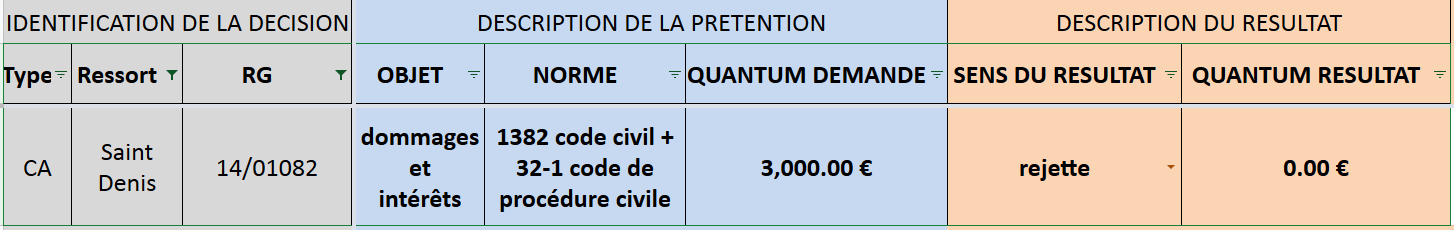
\includegraphics[width=\textwidth]{tab-danais.png}
	\caption{\scriptsize Informations à extraire (dommages-intérêts pour procédure abusive)}
\end{table}
\end{frame}

\subsection{Méthode : identifier les passages, puis les informations}

\begin{frame}[c]{Retrouver les demandes à l'aide des termes clés}
		\fbox{\parbox{\textwidth}{
				" ... 
				
				- débouter M. S. de ... % l' ensemble de ses demandes
				
				- le \underline{condamner} à payer une \textbf{amende civile} de  \textit{1.500 euros} \textbf{pour procédure abusive} ...
				
				- le \underline{condamner} à payer la somme ..."
		}}
\end{frame}
\subsection{Expérimentations sur 6 catégories de demandes}
\begin{frame}{Données}
	\begin{figure}[!htb]
		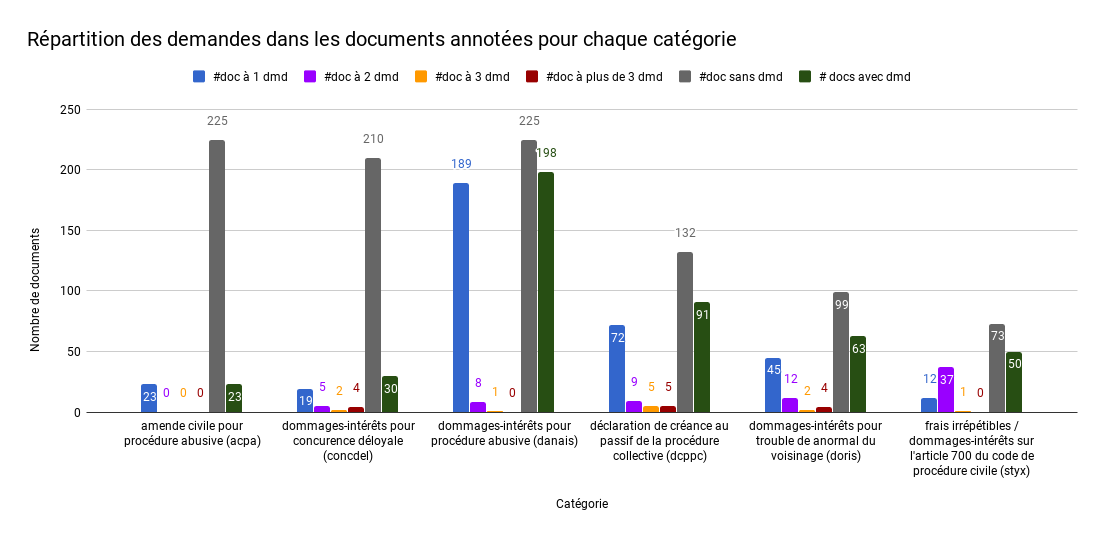
\includegraphics[width=0.8\textwidth]{chartDataset.png}
		\caption{\tiny Répartitions des demandes dans les documents annotées.}\label{fig:quanta:hist-repartition-docs}
	\end{figure}	
\end{frame}